%% LyX 2.3.4.2 created this file.  For more info, see http://www.lyx.org/.
%% Do not edit unless you really know what you are doing.
\documentclass[english,dvipsnames,aspectratio=169]{beamer}
\usepackage{mathptmx}
\usepackage{eulervm}
\usepackage[T1]{fontenc}
\usepackage[latin9]{inputenc}
\usepackage{babel}
\usepackage{amstext}
\usepackage{amssymb}
\usepackage{graphicx}
\usepackage{ifthen}
\usepackage{xcolor}
\usepackage{xspace}
\usepackage{tikz}
\usetikzlibrary{tikzmark}
\usetikzlibrary{calc}
\usepackage{pgfplots}
%\pgfplotsset{compat=1.17}
\usepackage{booktabs}
\usepackage{xpatch}

\xpatchcmd{\itemize}
  {\def\makelabel}
  {\ifnum\@itemdepth=1\relax
     \setlength\itemsep{2ex}% separation for first level
   \else
     \ifnum\@itemdepth=2\relax
       \setlength\itemsep{1ex}% separation for second level
     \else
       \ifnum\@itemdepth=3\relax
         \setlength\itemsep{0.5ex}% separation for third level
   \fi\fi\fi\def\makelabel
  }
 {}
 {}

\ifx\hypersetup\undefined
  \AtBeginDocument{%
    \hypersetup{unicode=true,pdfusetitle,
 bookmarks=true,bookmarksnumbered=false,bookmarksopen=false,
 breaklinks=false,pdfborder={0 0 0},pdfborderstyle={},backref=false,colorlinks=true,
 allcolors=NYUPurple,urlcolor=LightPurple}
  }
\else
  \hypersetup{unicode=true,pdfusetitle,
 bookmarks=true,bookmarksnumbered=false,bookmarksopen=false,
 breaklinks=false,pdfborder={0 0 0},pdfborderstyle={},backref=false,colorlinks=true,
 allcolors=NYUPurple,urlcolor=LightPurple}
\fi

\makeatletter

%%%%%%%%%%%%%%%%%%%%%%%%%%%%%% LyX specific LaTeX commands.
%% Because html converters don't know tabularnewline
\providecommand{\tabularnewline}{\\}

%%%%%%%%%%%%%%%%%%%%%%%%%%%%%% Textclass specific LaTeX commands.
% this default might be overridden by plain title style
\newcommand\makebeamertitle{\frame{\maketitle}}%
% (ERT) argument for the TOC
\AtBeginDocument{%
  \let\origtableofcontents=\tableofcontents
  \def\tableofcontents{\@ifnextchar[{\origtableofcontents}{\gobbletableofcontents}}
  \def\gobbletableofcontents#1{\origtableofcontents}
}

%%%%%%%%%%%%%%%%%%%%%%%%%%%%%% User specified LaTeX commands.
\usetheme{CambridgeUS} 
\beamertemplatenavigationsymbolsempty


% Set Color ==============================
\definecolor{NYUPurple}{RGB}{87,6,140}
\definecolor{LightPurple}{RGB}{165,11,255}


\setbeamercolor{title}{fg=NYUPurple}
\setbeamercolor{frametitle}{fg=NYUPurple}

\setbeamercolor{background canvas}{fg=NYUPurple, bg=white}
\setbeamercolor{background}{fg=black, bg=NYUPurple}

\setbeamercolor{palette primary}{fg=black, bg=gray!30!white}
\setbeamercolor{palette secondary}{fg=black, bg=gray!20!white}
\setbeamercolor{palette tertiary}{fg=gray!20!white, bg=NYUPurple}

\setbeamertemplate{headline}{}
\setbeamerfont{itemize/enumerate body}{}
\setbeamerfont{itemize/enumerate subbody}{size=\normalsize}

\setbeamercolor{parttitle}{fg=NYUPurple}
\setbeamercolor{sectiontitle}{fg=NYUPurple}
\setbeamercolor{sectionname}{fg=NYUPurple}
\setbeamercolor{section page}{fg=NYUPurple}
%\setbeamercolor{description item}{fg=NYUPurple}
%\setbeamercolor{block title}{fg=NYUPurple}

\setbeamertemplate{blocks}[rounded][shadow=false]
\setbeamercolor{block body}{bg=normal text.bg!90!NYUPurple}
\setbeamercolor{block title}{bg=NYUPurple!30, fg=NYUPurple}



\AtBeginSection[]{
  \begin{frame}
  \vfill
  \centering
\setbeamercolor{section title}{fg=NYUPurple}
 \begin{beamercolorbox}[sep=8pt,center,shadow=true,rounded=true]{title}
    \usebeamerfont{title}\usebeamercolor[fg]{title}\insertsectionhead\par%
  \end{beamercolorbox}
  \vfill
  \end{frame}
}

\makeatother

\setlength{\parskip}{\medskipamount} 

\input ../macros

\begin{document}
\input ../rosenberg-macros

\title[DS-GA 1003]{What is Machine Learning}
\author{Mengye Ren
}
% \vspace{2em}{
%     Slides based on David Rosenberg and He He's materials
%     % Lecture \href{https://davidrosenberg.github.io/mlcourse/Archive/2017Fall/Lectures/01.black-box-ML.pdf}{1}
%     % from David Rosenberg's \href{https://github.com/davidrosenberg/mlcourse}{course material}.
% }

\date{September 5, 2023}
\institute{NYU}

\makebeamertitle
\mode<article>{Just in article version}

\begin{frame}{Machine Learning Problems}

We'll start with a few canonical examples.
\end{frame}
%
\begin{frame}{What is learning?}
  \textit{ "The activity or process of gaining knowledge or skill by studying, practicing, being taught, or experiencing something."
    \begin{flushright}Merriam Webster dictionary\end{flushright}}
  \pause
  \vspace{1em}
  \textit{ ``A computer program is said to \emph{learn} from experience E with respect to some class of tasks T and performance measure P, if its performance at tasks in T, as measured by P, improves with experience E.''
  \begin{flushright}Tom Mitchell\end{flushright}}
\end{frame}

\begin{frame}{Applications of machine learning}
  \begin{itemize}
  \setlength\itemsep{1em}
  \item For many problems, it's difficult to program the correct behavior by hand
    \begin{itemize}
    \item recognizing people and objects
    \item understanding human speech
    \end{itemize}
    \pause
    \item Machine learning approach: program an algorithm to automatically learn from data, or from experience. Typically our goal is to solve a prediction problem of the format:
    \begin{itemize}
    \item Given an \textbf{input} $x$,
    \item \textbf{Predict} an \textbf{output $y$.} 
    \end{itemize}

    \pause
  \item Why might you want to use a learning algorithm?
    \pause
    \begin{itemize}
    \item hard to code up a solution by hand (e.g.~vision, speech)
    \item system needs to adapt to a changing environment (e.g.~spam detection)
    \item want the system to perform \emph{better} than the human programmers
    \item privacy/fairness (e.g.~ranking search results)
    \end{itemize}
  \end{itemize}
\end{frame}

\begin{frame}{Example: Spam Detection}

\begin{itemize}
\item \textbf{Input x:} Incoming email
\end{itemize}
\begin{center}
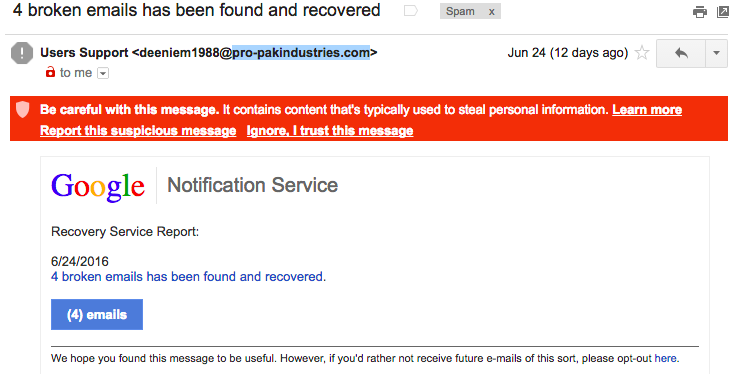
\includegraphics[width=0.6\textwidth]{figures/spam-email}
\end{center}

\begin{itemize}
\item \textbf{Output y: }``SPAM'' or ``NOT SPAM''
\item This is a \textbf{binary classification} problem: there are two 
possible outputs.
\end{itemize}
\end{frame}

\begin{frame}{Example: Medical Diagnosis}
\begin{itemize}
\item \textbf{Input x:} Symptoms (fever, cough, fast breathing, shaking, nausea, ...)

\item \textbf{Output y:} Diagnosis (pneumonia, flu, common cold, bronchitis, ...)

\item A \textbf{multiclass classification} problem: choosing an output out of a \emph{discrete} set of possible outputs.
\end{itemize}

\medskip
How do we express uncertainty about the output?
\begin{itemize}
\item \textbf{Probabilistic classification} or \textbf{soft classification}:
\begin{eqnarray*}
\text{\ensuremath{\pr}(pneumonia)} & = & 0.7\\
\text{\ensuremath{\pr}(flu)} & = & 0.2\\
\vdots &  & \vdots
\end{eqnarray*}
\end{itemize}
\end{frame}

\begin{frame}{Example: Predicting a Stock Price}
\begin{itemize}
\item \textbf{Input x:} History of the stock's prices
\item \textbf{Output y:} The price of the stock at the close of the next day
\end{itemize}

\begin{itemize}
    \item This is called a \textbf{regression} problem (for historical reasons): the output is \emph{continuous}.
\end{itemize}

\end{frame}

\begin{frame}{Comparison to Rule-Based Approaches (Expert Systems)}
\begin{itemize}
\item Consider the problem of medical diagnosis.

\begin{enumerate}
    \item Talk to experts (in this case, medical doctors).
    \item Understand how the experts come up with a diagnosis.
    \item Implement this process as an algorithm (a \textbf{rule-based system}): e.g., a set of symptoms $\rightarrow$ a particular diagnosis.
    \item Potentially use logical deduction to infer new rules from the rules that are stored in the knowledge base.  
\end{enumerate} 
\end{itemize}
\end{frame}

\begin{frame}{Rule-Based Approach}
\begin{center}
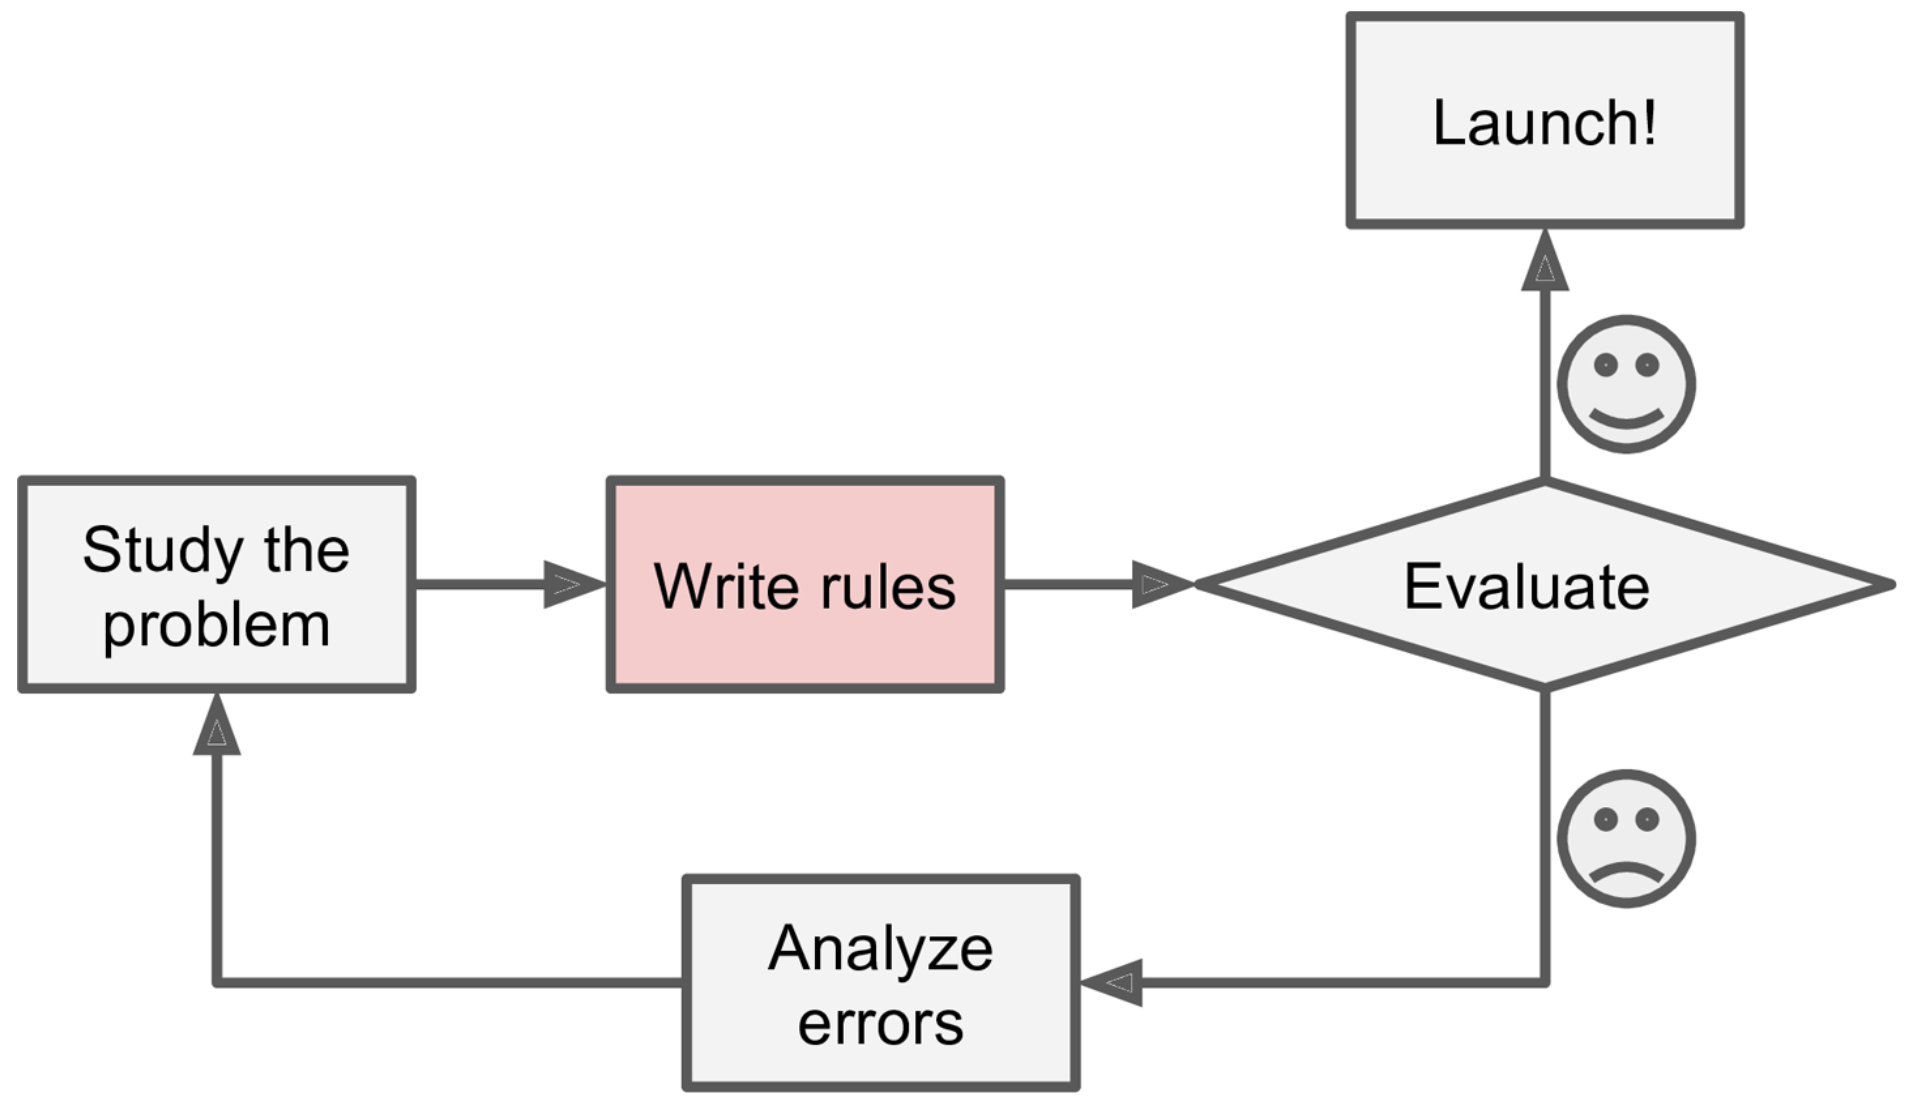
\includegraphics[height=0.7\textheight]{figures/geron-fig1-1}\let\thefootnote\relax\footnotetext{\tiny{Fig 1-1 from \emph{Hands-On Machine Learning with Scikit-Learn and TensorFlow} by Aurelien Geron (2017).}}
\par\end{center}

\end{frame}

\begin{frame}{Advantages of Rule-Based Approaches}
\begin{itemize}
    \item Leverage existing domain expertise.
    \item Generally \textbf{interpretable}: We can describe the rule to another human
    \item Produce reliable answers for the scenarios that are included in the knowledge bases.
\end{itemize}
\end{frame}

\begin{frame}{Limitations of Rule-Based Systems}

\begin{itemize}
\item Labor intensive to build: experts' time is expensive.
\item Rules work very well for areas they cover, but often do not \textbf{generalize} to unanticipated input combinations.
\item Don't naturally handle uncertainty.
\end{itemize}
\end{frame}

\begin{frame}{The Machine Learning Approach}
\begin{itemize}
    \item Instead of explicitly engineering the process that a human expert would use to make the decision...

    \item We have the machine \textbf{learn} on its own from inputs and outputs (decisions).

\item We provide \textbf{training data}:
many examples of (input $x$ , output $y$) pairs, e.g.

\begin{itemize}
\item A set of videos, and whether or not each has a cat in it.
\item A set of emails, and whether or not each one should go to the spam folder.
\end{itemize}

\item Learning from training data of this form (inputs and outputs) is called \textbf{supervised learning}.
\end{itemize}
\end{frame}

\begin{frame}{Machine Learning Algorithm}
\begin{itemize}
\item A \textbf{machine learning algorithm} learns from the training data:
\begin{itemize}
\item \textbf{Input}: Training Data (e.g., emails $x$ and their labels $y$)
\item \textbf{Output}: A prediction function that produces output
$y$ given input $x$.
\end{itemize}

\item The goal of machine learning is to find the ``best'' (to be defined) prediction function \textbf{automatically, based on the training data}
%

\item The success of ML depends on
    \begin{itemize}
        \item The availability of large amounts of data;
        \item \textbf{Generalization} to unseen samples (the test set): just memorizing the training set will not be useful.
    \end{itemize}
\end{itemize}
\end{frame}

\begin{frame}{Machine Learning Approach}
\begin{center}
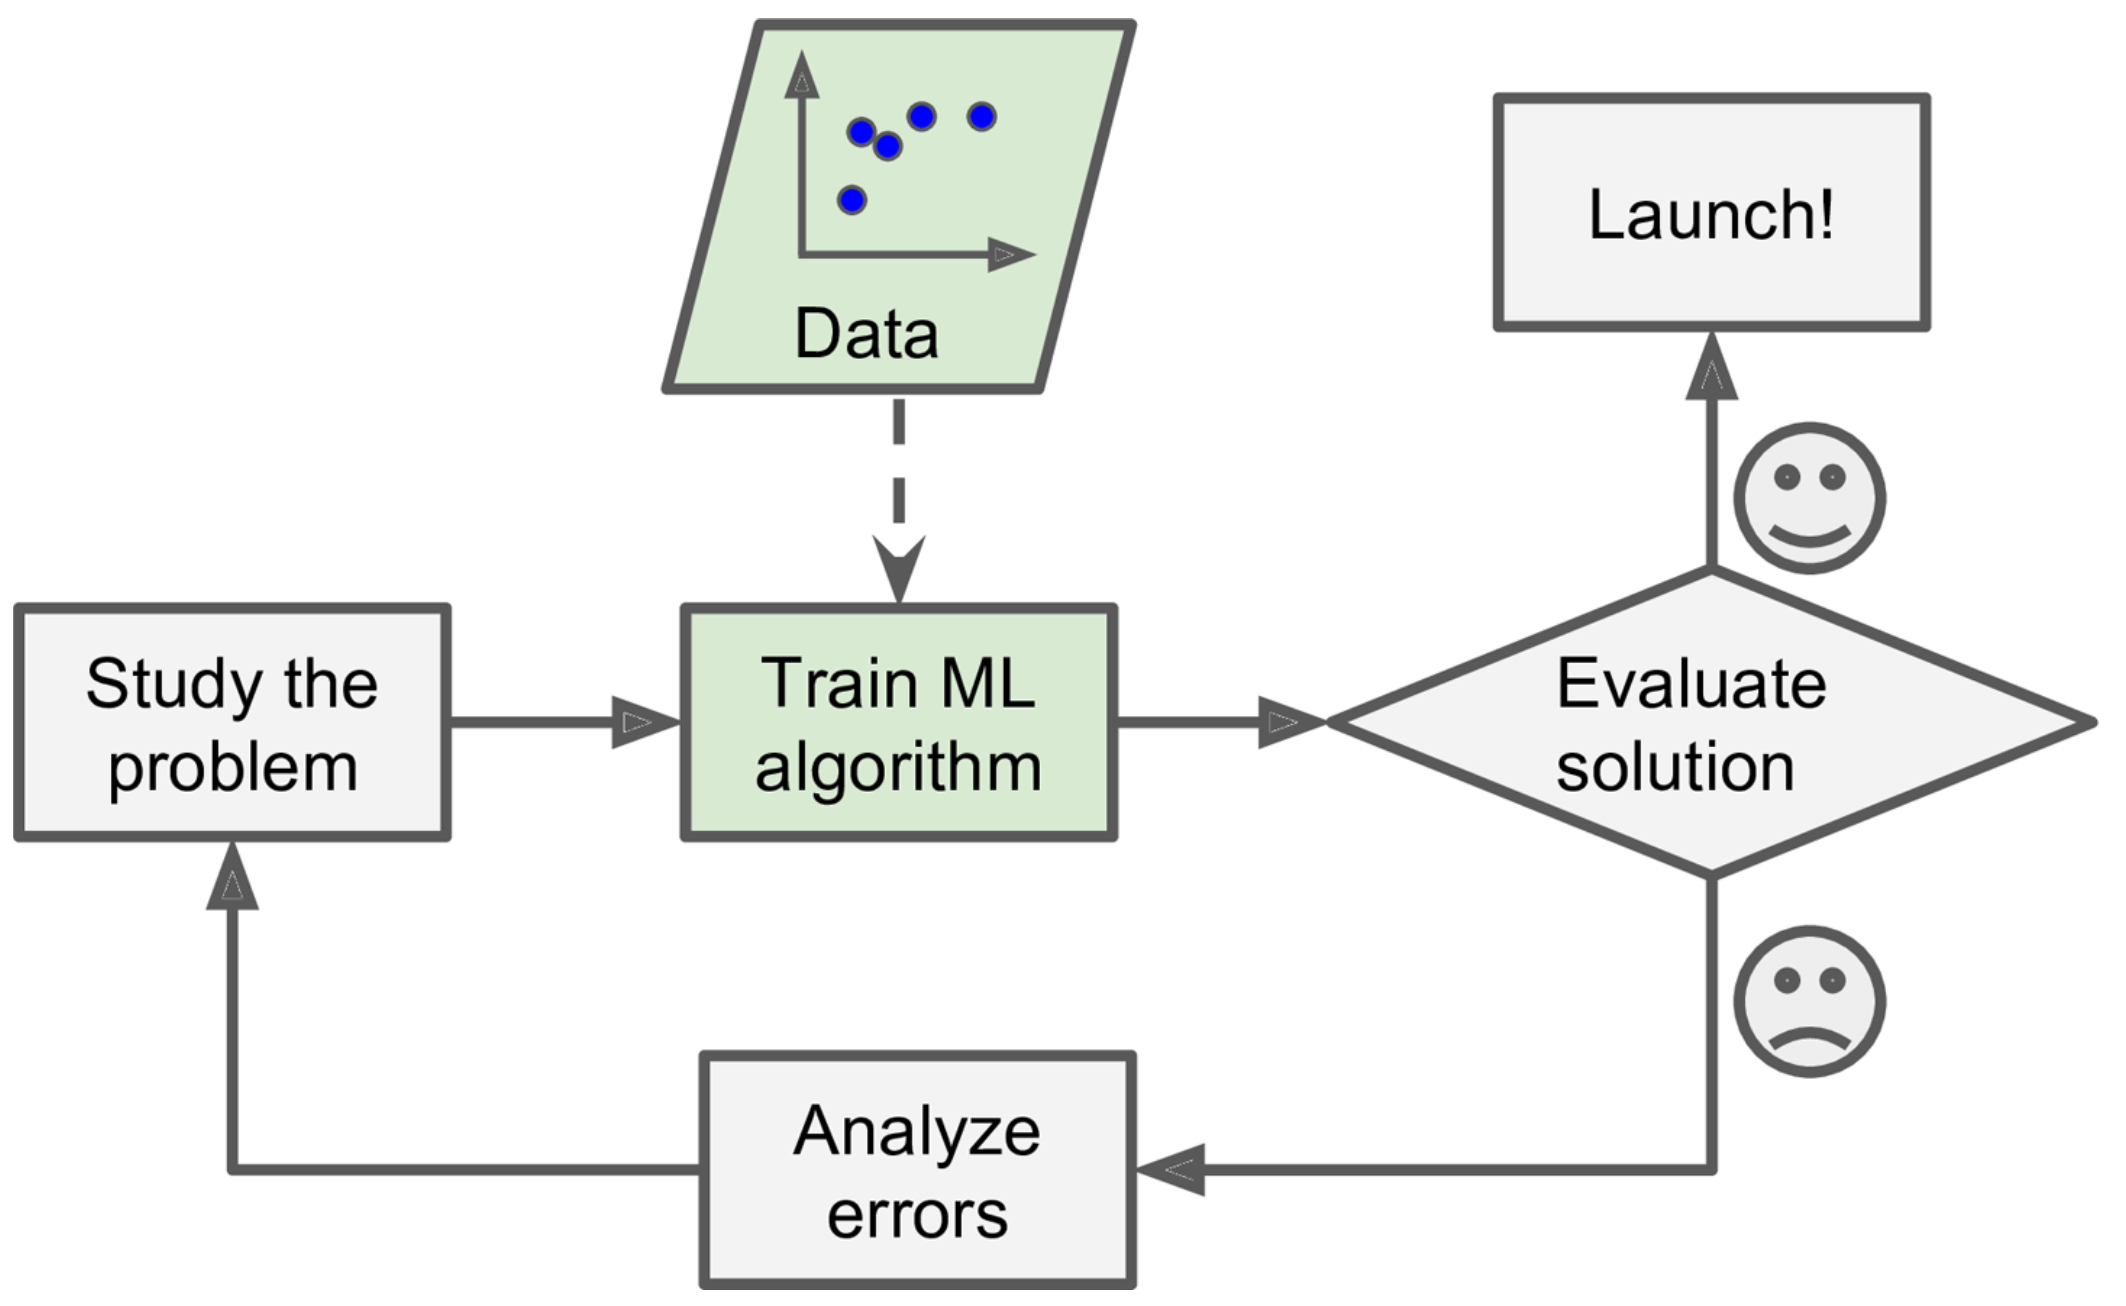
\includegraphics[height=0.7\textheight]{figures/geron-fig1-2}
\par\end{center}

\mode<article>{We've swapped out rule writing with ``machine learning.'' But how
does adjust the ML training process by analyzing errors?}
\begin{center}
\let\thefootnote\relax\footnotetext{\tiny{Fig 1-2 from \emph{Hands-On Machine Learning with Scikit-Learn and TensorFlow} by Aurelien Geron (2017).}}
\par\end{center}

\end{frame}

\begin{frame}{Key concepts}
    \begin{itemize}[<+->]
    \item The most common \textbf{ML problem types}:

\begin{itemize}
    \item Classification (binary and multiclass)
\item Regression
\end{itemize}

\item \textbf{Prediction function}: predicts output $y$ (e.g. spam or not?) given input $x$ (e.g. email)
\item \textbf{Training data}: a set of (input $x$, output $y$) pairs
\item \textbf{Supervised learning algorithm}: takes training data and produces a prediction function
\item Beyond prediction
    \begin{itemize}
        \item \textbf{Unsupervised learning}: finding structures in data, e.g. clustering
        \item \textbf{Reinforcement learning}: optimizing long-term objective, e.g. Go  
        \item \textbf{Representation learning}: learning good features of real-world objects, e.g. text
    \end{itemize}
\end{itemize}
\end{frame}

\begin{frame}
    {Core Questions in Machine Learning}
    Given any task, the following questions need to be answered:
    \begin{itemize}
        \item \textbf{Modeling}: What class of prediction functions are we considering?
        \item \textbf{Learning}: How do we learn the ``best'' prediction function in this class from our training data?
        \item \textbf{Inference}: How do we compute the output of the prediction function for a new input?
    \end{itemize}
\end{frame}

\end{document}
